%This is a template for PHYS 546 papers based on the
%APS template.aps file for REVTeX 4.  All lines (like this one) that
%begin with a "%" are comments.
%\documentclass[aps,preprint,groupedaddress,letterpaper]{revtex4}
\documentclass[aps,twocolumn,groupedaddress]{revtex4}
\usepackage{graphicx}
\usepackage{bm}
\usepackage{hyperref}

\begin{document}

\title{Magnetic Properties of Recording Media in Magnetic Storage Devices}

\author{Louis Coleman}
\affiliation{Department of Physics \& Astronomy, California State University, Long Beach, Long Beach, CA 90840}

\begin{abstract}
Magnetic properties of recording media (RM) from a cassette tape and floppy disk as well as a Samarium-Iron-Permalloy (SmFePy) thin film were acquired using an Alternating Gradient Magnetometer (AGM). Fields from +/- 1000 Oe to +/- 1600 Oe were applied to the samples giving material specific Hysteresis loops and FORC diagrams of the samples. The Hysteresis loops and FORC diagrams shed light on the samples data integrity and what applications the samples can be used in. The floppy disk and cassette tape have the highest respective coercivities and the lowest respective squareness ratios. For the recording media, the floppy disk is prone to self-demagnetization although the cassette tape is inclined to flipping magnetization from random magnetic fields. The SmFePy is significantly more prone to arbitrary magnetic fields, but not magnetic domain instability.
\end{abstract}

%%%% Make sure that \maketitle command is after the abstract
\maketitle

\section{Introduction}
In 1878, Oberlin Smith created the first known magnetic storage device for audio recordings. The storage capabilities of magnetic media have evolved to allow storing digital copies of video, audio, pictures, software, and other forms of data.  Magnetic storage has advanced to have higher data density, integrity, and requires less energy to store the same amount of information generation after generation.

Most magnetic media consist of a ferromagnetic material on a non-magnetic substrate. The magnetic domains in the ferromagnetic layer orient their magnetic moments a particular direction to read as a 1 or 0 in digital media, while in audio tape the magnitude of the remnant magnetization corresponds to a particular frequency of an audio recording. The application a particular magnetic media is suited for depends on the category of the magnetic layer. ''Hard'' magnetic material is used in video, audio, and data applications. They have higher coercive fields, remanence, and wider hysteresis loops making it more difficult to switch the magnetic polarization or demagnetize the material do to stray magnetic fields. Squareness and coercivity squareness ratios being tied to data integrity further distinguish the differences between forms of magnetic storage. Having a higher squareness prevents errors from thermal fluctuations. ''Soft'' magnetic material is used in transformer or other electromagnetic cores. They have a lower coercive force and reverse magnetization direction without dissipating much energy \cite{LEWIS}. The energy loss is related to the area of the hysteresis loop and the movement of domain walls. 

An alternating gradient magnetometer (AGM) measures the magnetic properties of a cassette tape RM, floppy disk RM, and Samarium-Iron-Permalloy (SmFePy) thin film, while the accompanying software provides Hysteresis loop diagrams and first order reversal curves (FORCs). The FORCinel software converts the FORC curves into FORC diagrams using a locally-weighted regression smoothing technique used by Harrison and Feinberg (2008)  \cite{HARRISON}.

\section{Theory}
Atomic dipoles of ferromagnetic material align themselves to an applied magnetic field. Applying a strong enough field strength aligns all the domains of the material to the external field giving a total magnetic moment or saturation magnetization $M_s$. When the applied field vanishes a magnetization remains known as the remanent magnetization $M_r$. The applied field’s magnitude necessary to demagnetize the material from saturation is the coercivity $H_c$, however a material can be demagnetized from thermal vibrations over time as well. Taking a material from positive saturation to negative saturation over a range of applied magnetic fields gives a diagram closely following the Preisach-Neel model of hysteresis. The squareness of the hysteresis loop indicates the strength of the read signal and is proportional to the remanence.

\begin{equation}
S= M_r / M_s
\label{squareness}
\end{equation}	

The coercivity squareness is given by

\begin{equation}
S^* = 1- M_r / \chi_0 H_c
\label{coercivesquareness}
\end{equation}	

And is an indicator of the strength needed to erase and write the data. $\chi_0$ being the magnetic susceptibility of the material. Both squareness ratios have a value from 0 to 1. Material with higher squareness ratios have less of a problem with self- demagnetization from thermally activated domain wall motion and repulsive forces between domains \cite{NAKAGAWA}. 

FORC curves follow the methodology of the hysteresis loop. However, after a specimen is subjected to a saturation field, the field is lowered to a characteristic field strength $H_a$ and then progressively saturated again at incremental field steps of $H_b$. The process is repeated for many values of $H_a$ with regular spacing between steps of $H_a$ and $H_b$ giving the measured magnetization $M(H_a, H_b)$. The FORC distribution is obtained from the second derivative of the magnetization

\begin{equation}
\rho(H_a, H_b ) =\partial^2 M(H_a , H_b )/ \partial H_a \partial H_b 
\label{coercivesquareness}
\end{equation}

To plot as a contour there is a coordinate transformation from $(H_a, H_b)$ to $H_c = (H_b –- H_a)/2$ and $H_\mu = (H_b ++ H_a)/2$, where $H_\mu$ is the particulate interaction field. The FORC diagram obtained is not a slightly distorted distribution of the Preisach function and should not be confused with a Preisach diagram \cite{DOBROTA}. FORC diagrams are sensitive to magnetostatic interactions \cite{MUXWORTHY}. Identifying features such as shape of central peaks, tails, and more help in determining the material being studied such as whether the material consist of single domains, multiple domains, orientation of domains and more.

\section{Experiment}
Sections of cassette tape and floppy disk approximately 10 nm by 10 nm and a SmFePy thin film were obtained. The recording media of the cassette tape has a Mylar substrate, while that of the floppy disk contained a 2 $\mu$m layer of magnetic iron oxide deposited on a Mylar substrate. The total thickness of the floppy disk is about 70 $\mu$m. First, the MicroMag™ Model 2900 (AGM) was calibrated using a 605 $\mu$emu nickel foil standard giving a mechanical quality factor of 19. It then measured the magnetic moment of the samples at varying external magnetic field intensities taking hysteresis loop and FORCs measurements using the AGM 2011 software. Acoustic noise around the AGM was kept to a minimum. The applied fields ranged between +/- 1200 Oe (cassette tape), +/- 1500 Oe (floppy disk), and +/- 1000 Oe (SmFePy) for the hysteresis measurement, while the FORC measurements ranged between +/- 1500 Oe (cassette tape) and +/- 1600 Oe (floppy disk).

FORCinel v1.2.1 software processed the FORC diagram using the FORC curves.\\

\begin{figure}[h]
\includegraphics[width=2.0in]{aparatus}
\caption{AGM Apparatus}
\end{figure}

\section{Results}
\subsection{Hysteresis Loop}
\begin{figure}[h]
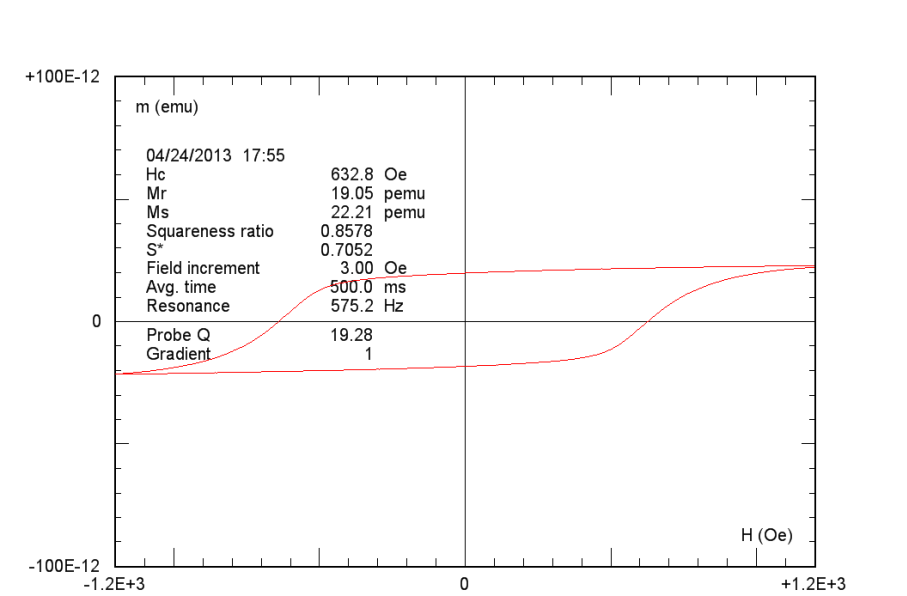
\includegraphics[width=3.3in]{cassettehyst}
\caption{Cassette Tape Hysteresis Loop. Direct Moment vs. Applied Magnetic Field Strength.}
\label{ch}
\end{figure}
\begin{figure}[h]
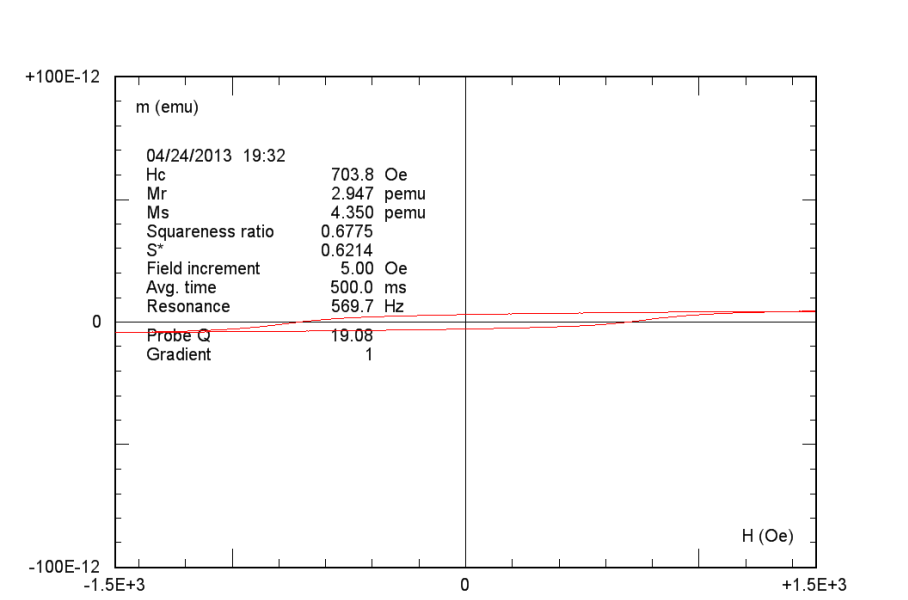
\includegraphics[width=3.3in]{floppyhyst}
\caption{Floppy Disk Hysteresis Loop. Direct Moment vs. Applied Magnetic Field Strength.}
\label{fh}
\end{figure}
\begin{figure}[h]
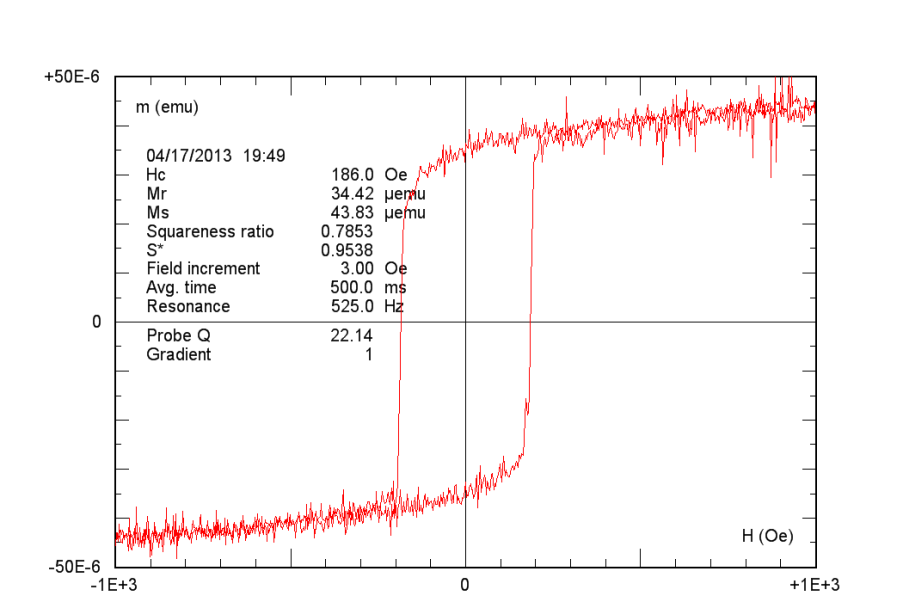
\includegraphics[width=3.3in]{smfepyhyst}
\caption{SmFePy Hysteresis Loop. Direct Moment vs. Applied Magnetic Field Strength.}
\label{sh}
\end{figure}
The hysteresis loop data for the cassette tape RM Fig.\ \ref{ch} , floppy disk RM Fig.\ \ref{fh}, and SmFePy Fig.\ \ref{sh} are represented. The coercivities are 632.8 Oe, 708.8 Oe, and 186.0 Oe respectively. The respective remanent magnetizations are 19.05 pemu, 2.947 pemu, and 34.42 $\mu$emu, while the magnetization saturations are a respective 22.21 pemu, 4.350 pemu, and 43.83 $\mu$emu. This give squareness ratios of 0.8578, 0.6775, and 0.7853, while the coercivity squareness ratios are 0.7052, 0.6214, and 0.9538 respectively. Additionally, the recording media has wide hysteresis loops compared to the SmFePy.

\subsection{FORC Diagrams}
\begin{figure}[h]
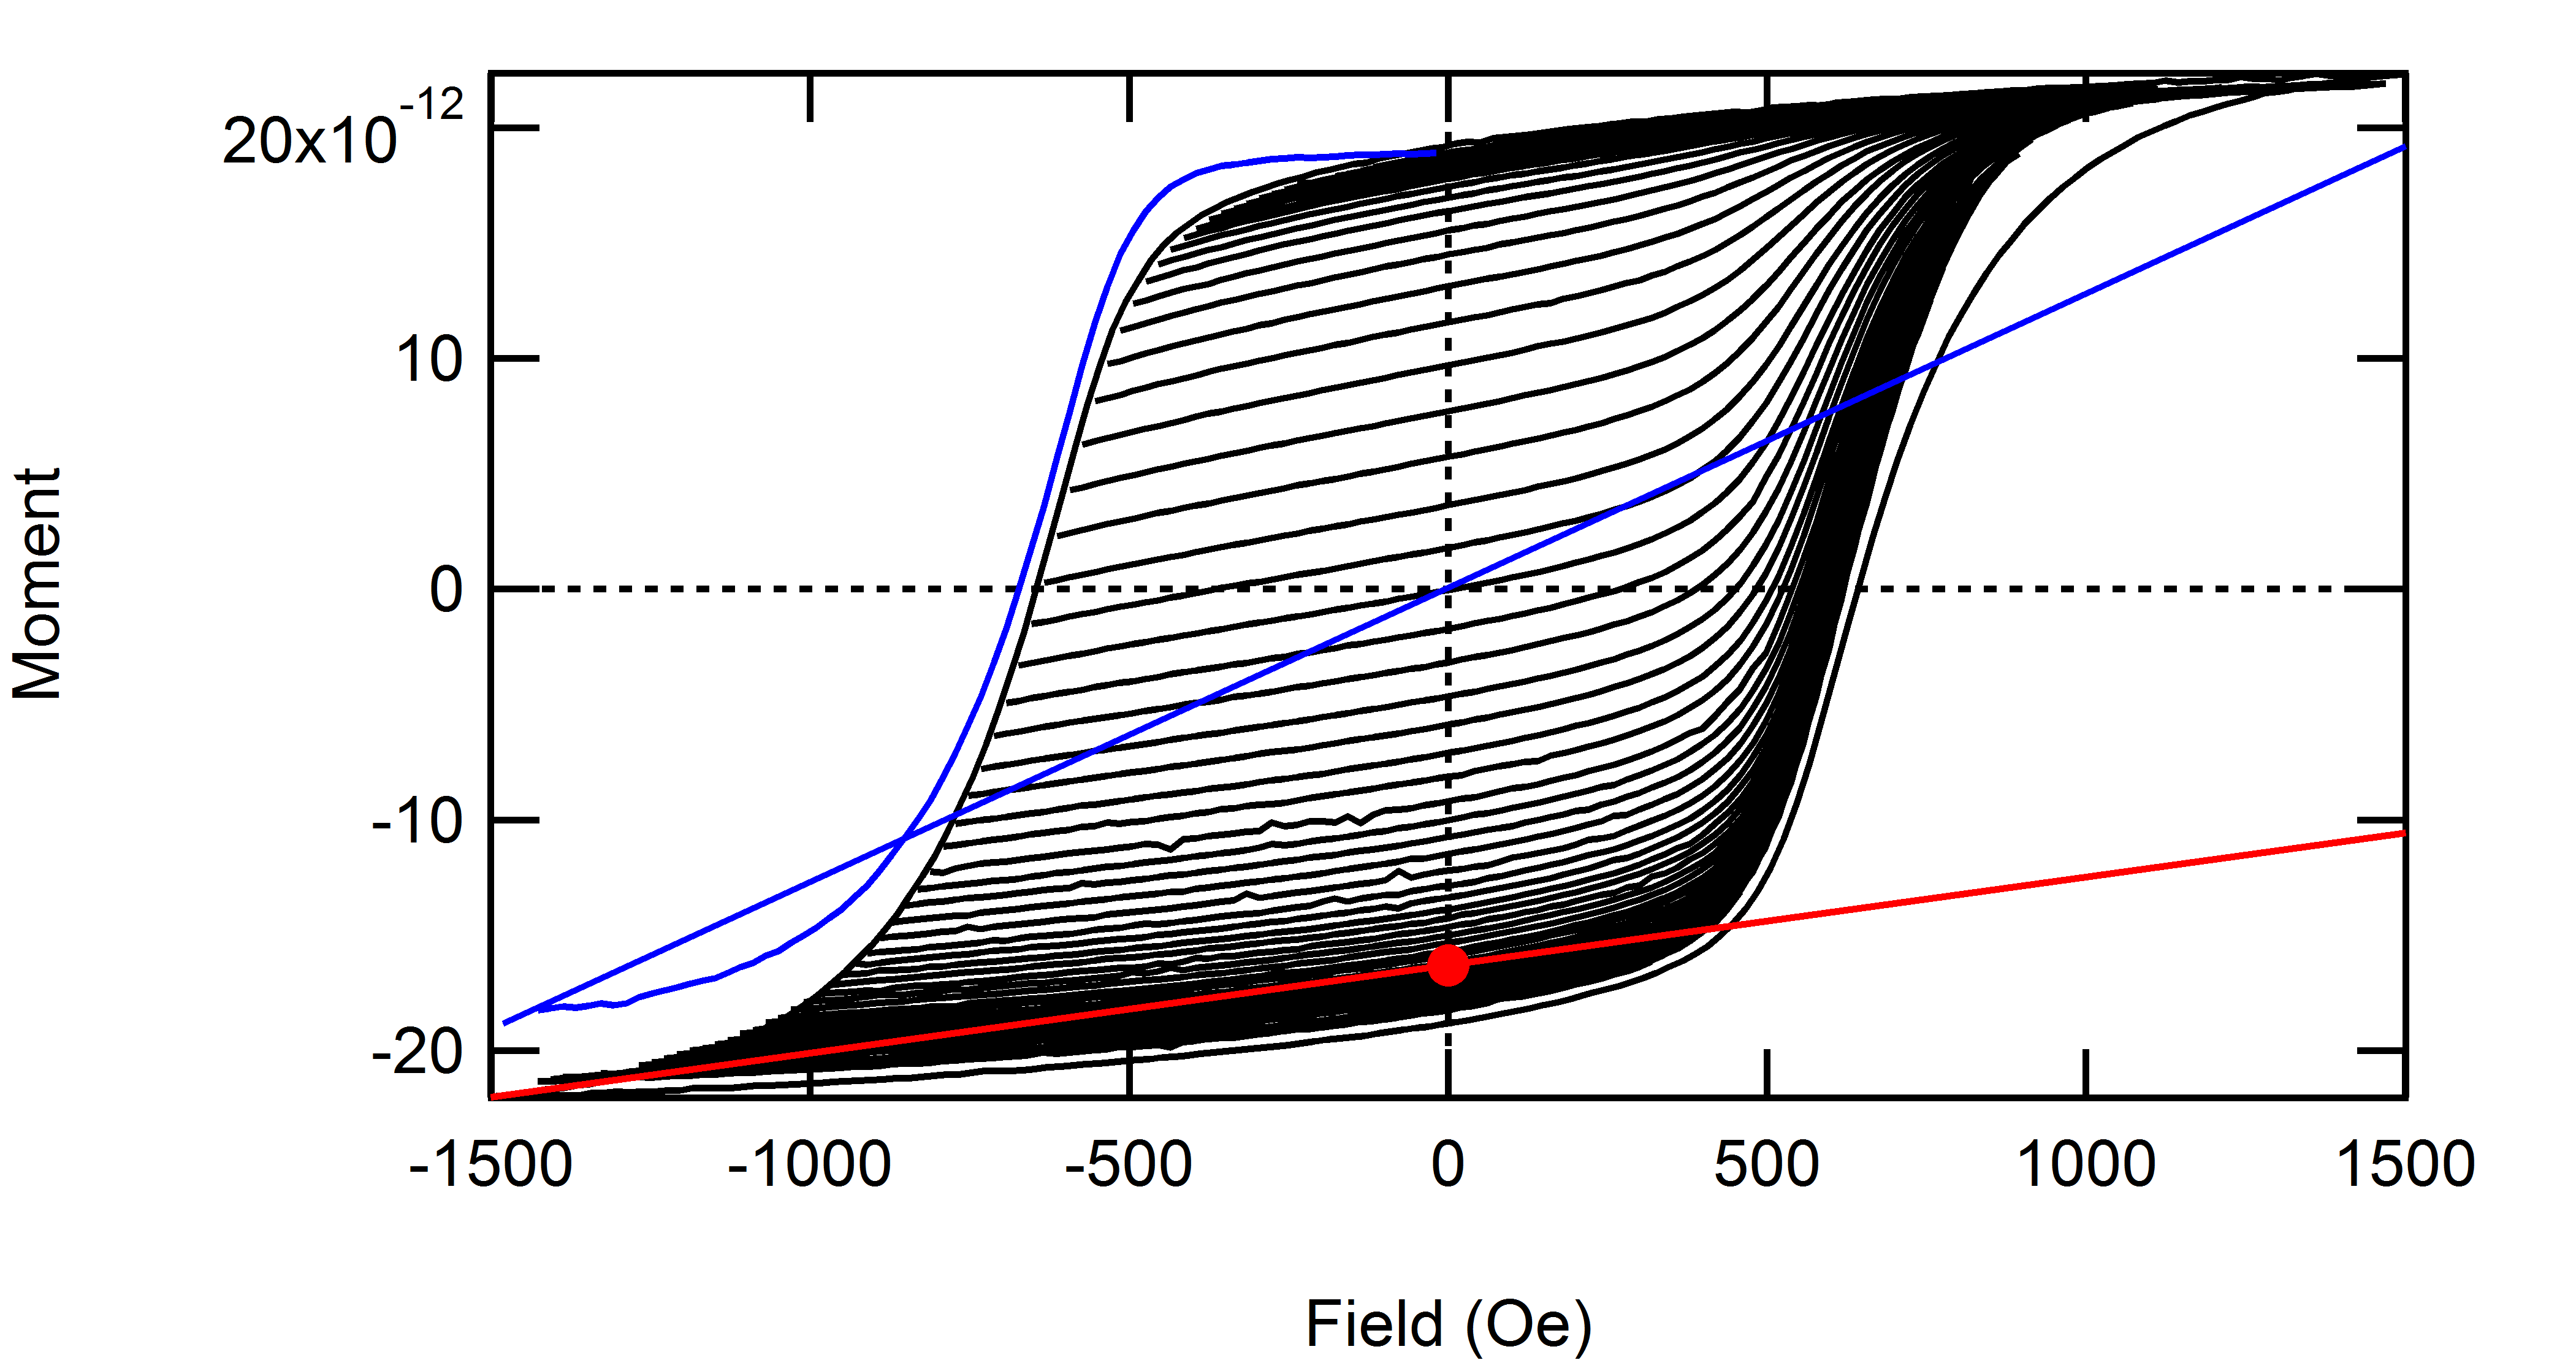
\includegraphics[width=3.3in]{cassetteforccurves}
\caption{Cassette Tape FORC Curves.}
\label{cff}
\end{figure}
\begin{figure}[h]
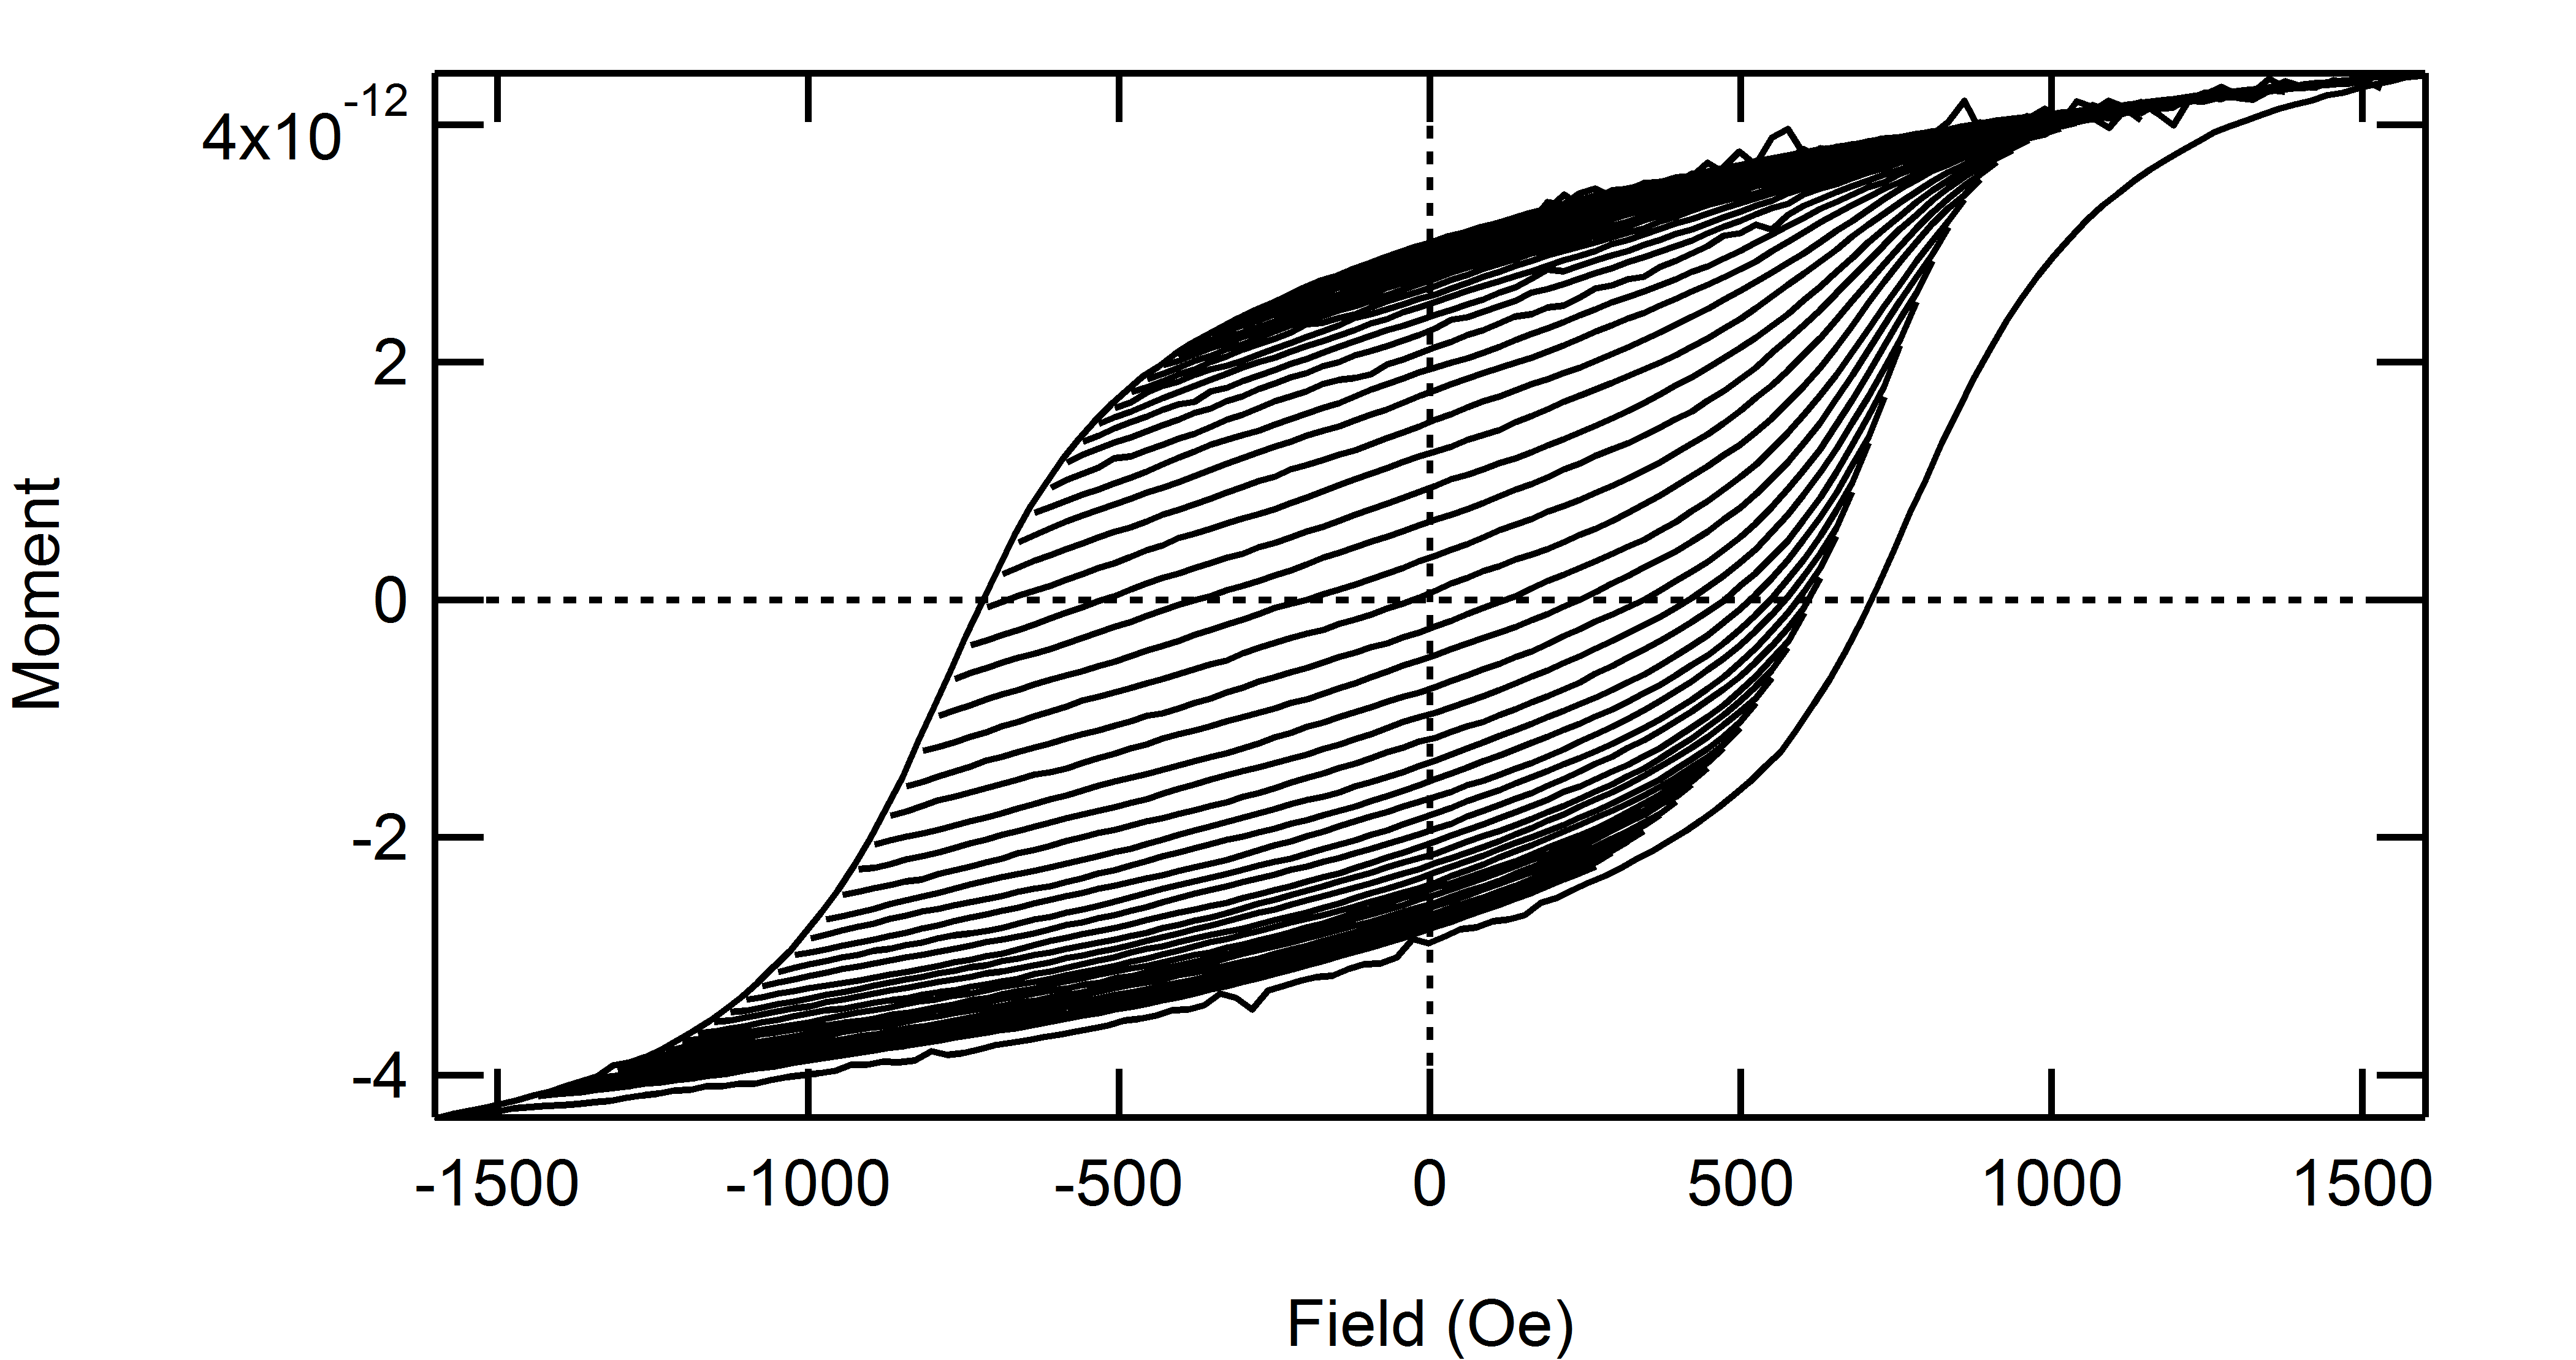
\includegraphics[width=3.3in]{floppyforccurves}
\caption{Floppy Disk FORC Curves.}
\label{fff}
\end{figure}
\begin{figure}[h]
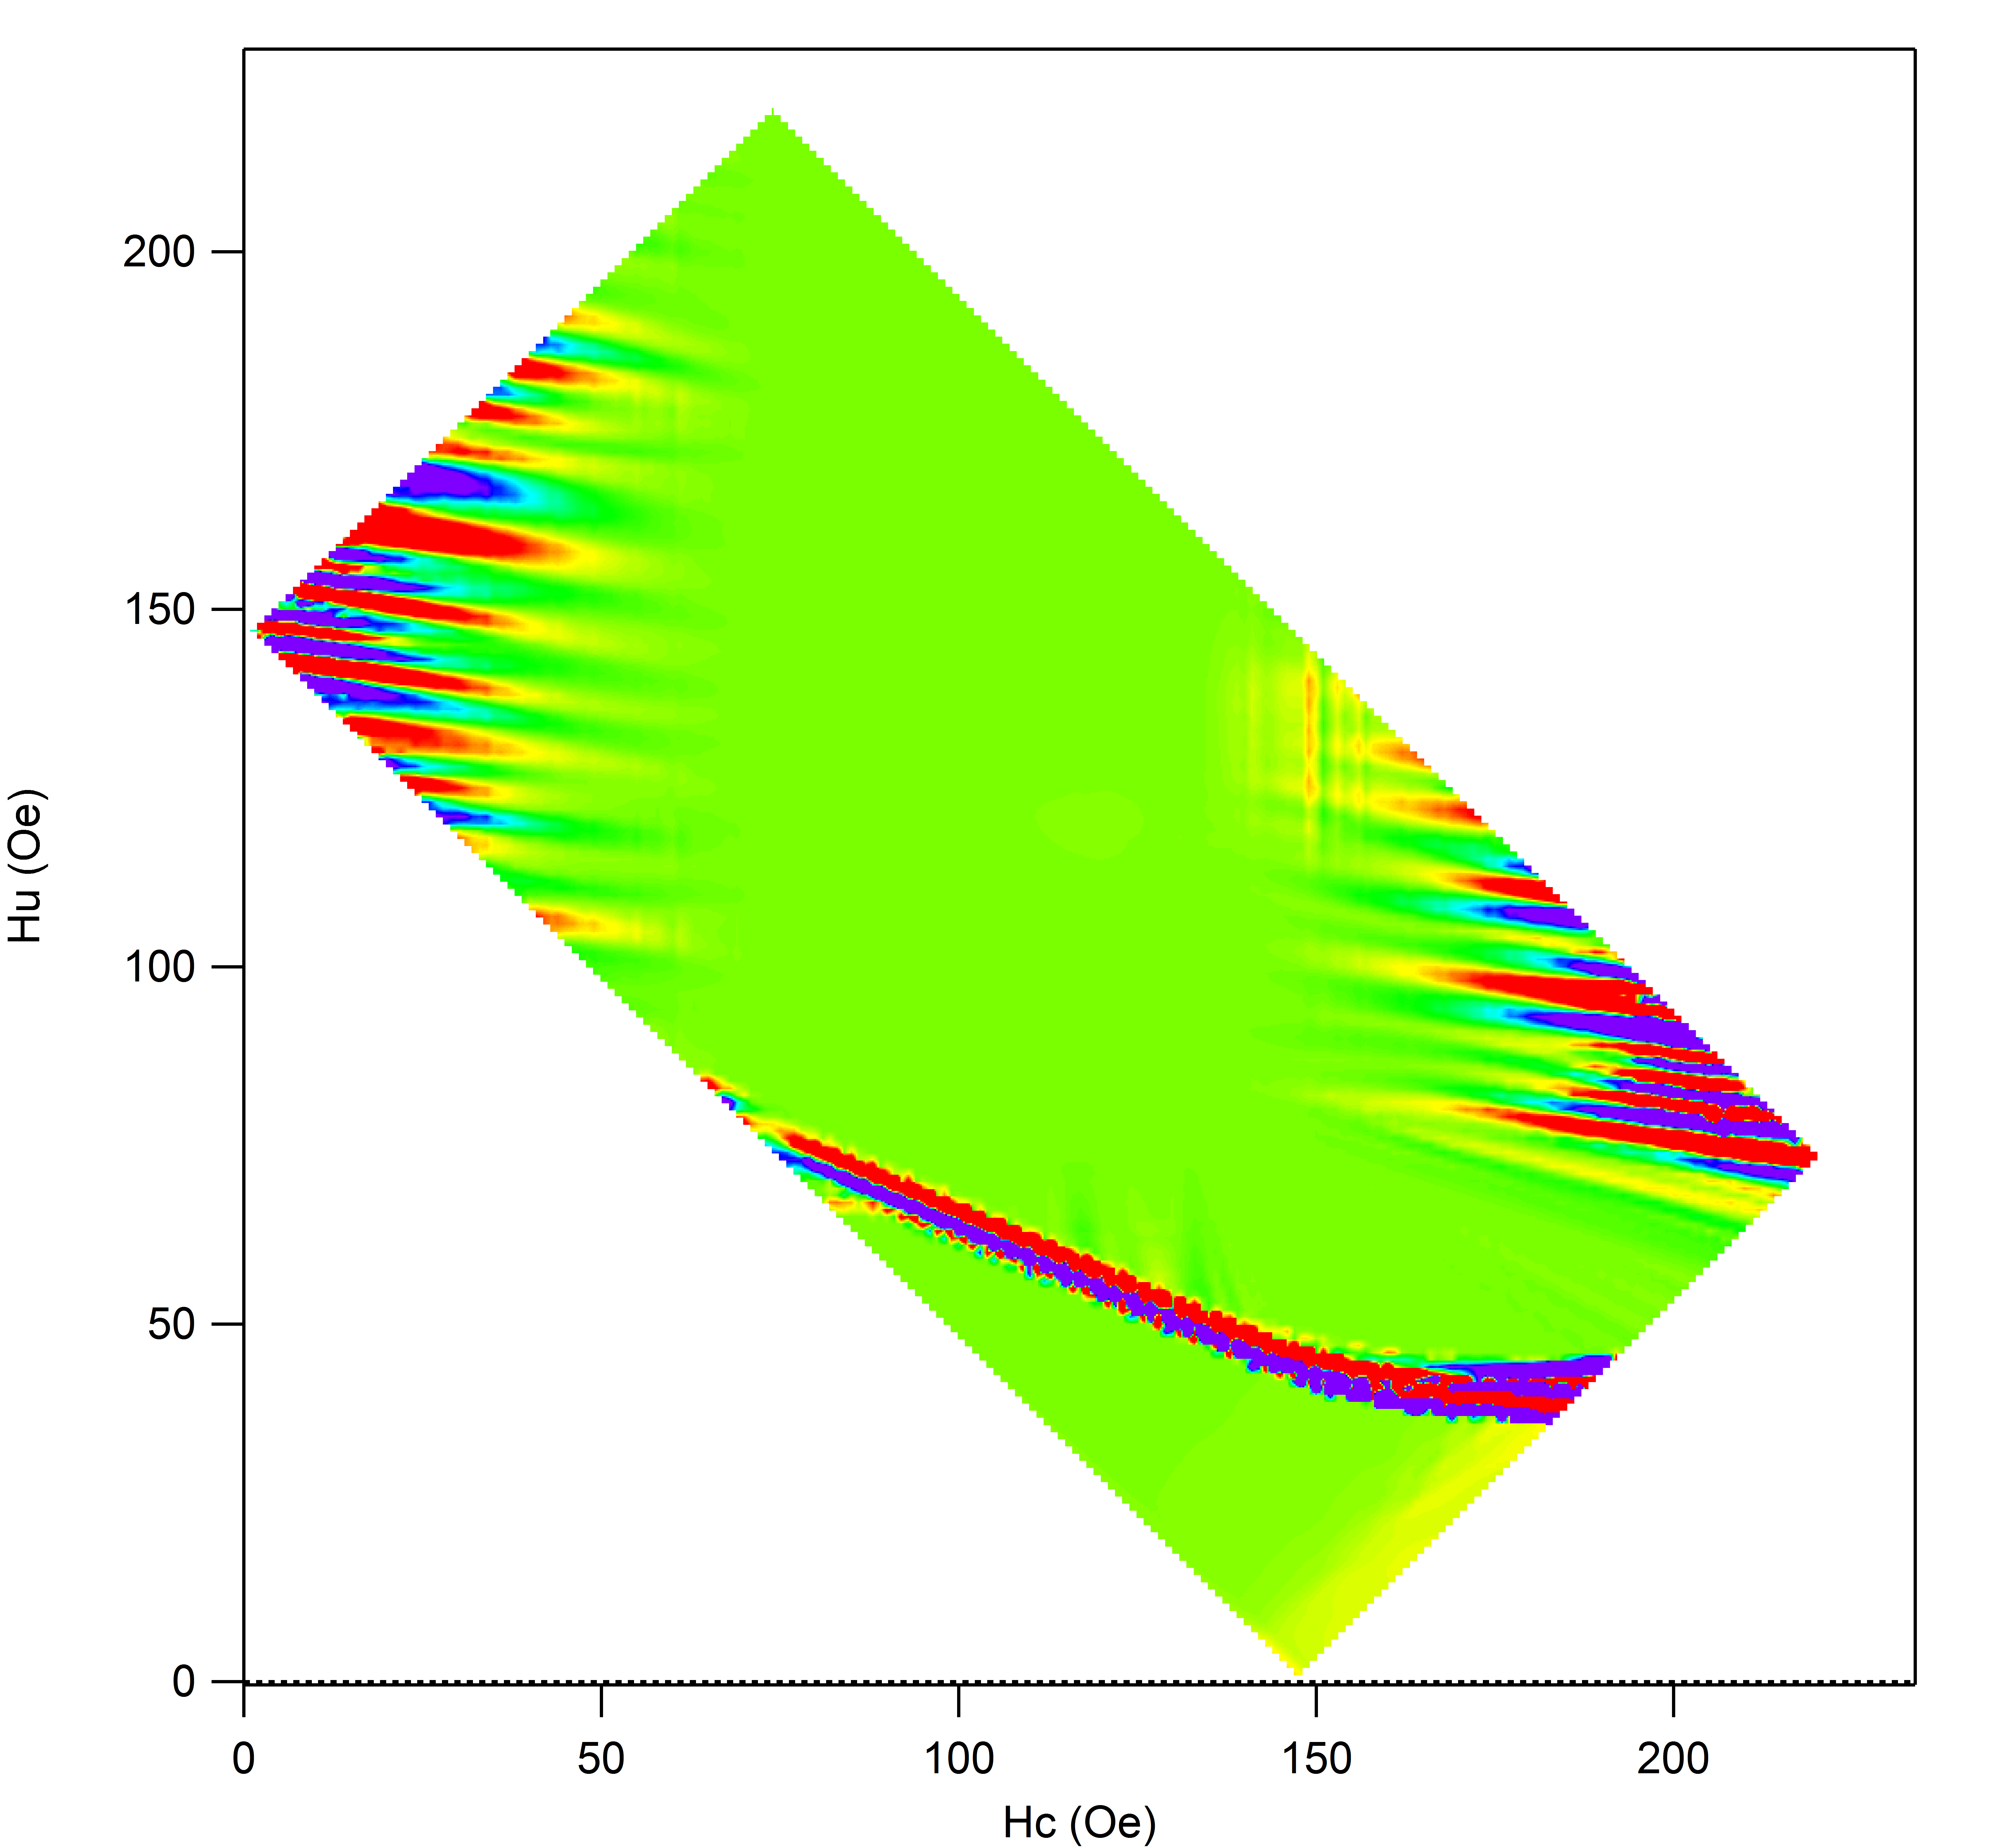
\includegraphics[width=3.3in]{cassetteforc}
\caption{Cassette Tape FORC Diagram.}
\label{cf}
\end{figure}
\begin{figure}[h]
\includegraphics[width=3.3in]{floppyforc}
\caption{Floppy Disk FORC Diagram.}
\label{ff}
\end{figure}
The FORC curves for the cassette tape RM Fig.\ \ref{cff} and floppy disk RM Fig.\ \ref{fff}. From these curves the FORC diagrams of the cassette tape RM Fig.\ \ref{cf} and floppy disk RM Fig.\ \ref{ff} are obtained.


\section{Discussion}
\subsection{Hysteresis Loop}
Both the floppy disk RM and cassette tape RM are in the range of ''hard'' media. The coercivities of both the floppy disk RM and cassette tape RM indicate they may be good for audio/video and data applications because of the large fields required to reverse their magnetic polarizations. The floppy disk RM requires higher fields and a greater dissipation of energy to both demagnetize and reverse the magnetization of its grains than the cassette tape RM. The squareness ratios indicate that the floppy disk has the greatest thermal instability or exchange interaction between neighboring magnetic domains making the stored data less reliable \cite{NAKAGAWA}. The magnetic moments of many domains will rotate to cancel out the inter-grain forces that repel each other, demagnetizing the material. This indicates that the floppy disk will need better error correction techniques to prevent corruption of data over time. The lower saturation magnetization is possibly because only a lower remanent magnetization is needed due to the smaller more sensitive read/write heads of floppy disk drives compared to the erase-record-reproduce heads of tape decks. 

The SmFePy suffers from a noisy signal due to acoustic noise; however, it is clear that it has ''soft'' magnetic properties and can be applied as the core in transformers and inducers based on its low coercive field. Like many permalloys it has a narrow, square hysteresis loop and a really high squareness ratio. The small dissipation of energy in switching magnetic polarization makes it ideal to reduce energy loss in electronic circuits with the reversing fields from AC current. Nevertheless, another testing of the material while eliminating all acoustic noise to get more accurate measurements of the coercivity and squareness ratios is a necessity.

\subsection{FORC Diagrams}
The FORC diagrams processed do not give the high point or eye of the contour plot due to the lack of data points obtained. A larger range of FORC curves at smaller increments of $H_a$ and $H_b$ must be obtained to acquire useful information from the contour plot. Determining the contribution of different or one magnetic material in the mixture could be determined by the symmetry or lack there of for the central peak. Being consisted of only one magnetic contributing material would give the center peak a circular symmetry, while consisting of more than one would produce an exchange spring system crunching the middle distribution. Having an asymmetric boomeranged center peak would mean that there are randomly oriented single domain grains \cite{MUXWORTHY}.

\section{Conclusion}
Hysteresis loops were acquired using an AGM for cassette tape recording media, floppy disk recording media, and a SmFePy thin film. FORC diagrams were processed from FORC curve data using FORCinel. The coercivities are 632.8 Oe, 708.8 Oe, and 186.0 Oe respectively, while the magnetization saturations are a respective 22.21 pemu, 4.350 pemu, and 43.83 $\mu$emu. The squareness ratios are 0.8578, 0.6775, and 0.7853, while the coercivity squareness ratios are 0.7052, 0.6214, and 0.9538 respectively. Both recording media are ''hard'' magnetic material, whereas the SmFePy is ''soft.'' The magnetic tape is less susceptible to self-demagnetization but more prone to stray magnetic fields than the floppy disk. The SmFePy dissipates less energy to flip magnetization, but has a lower chance of self-demagnetizing.

%Here is the list of cited works.
\begin{thebibliography}{}
\bibitem{MANUAL} ``MicroMag 2900 Alternating Gradient Magnetometer (AGM) Instruction Manual,'' Princeton Measurements Corporation, (2009)
\bibitem{HARRISON} R. J. Harrison and J. M. Feinberg, ``FORCinel: An improved algorithm for calculating first-order reversal curve distributions using locally weighted regression smoothing,'' GEOCHEMISTRY GEOPHYSICS GEOSYSTEMS, {\bf 9}, Q05016 (2008)
\bibitem{DOBROTA} C. Dobrota and A. Stancu, ``What does a first-order reversal curve diagram really mean? A study case: Array of ferromagnetic nanowires,'' J. Appl. Phys., {\bf 113},
043928 (2013)
\bibitem{FLANDERS} P. J. Flanders, ``An alternating gradient magnetometer,'' J. Appl. Phys., {\bf 63}, 3940 (1988)
\bibitem{NAKAGAWA} H. Nakagawa, H. Nemoto, Y. Honda, T. Ichihara, K. Tanahashi, and Y. Hosoe, ``Thermal stability and recording characteristics of TbCo/CoCrPt-hybrid media for perpendicular recording,'' J. Appl. Phys., {\bf 91}, 8016 (2002)
\bibitem{LEWIS} L. H. Lewis, J. Gao, D. C. Jiles, and D. O. Welch, ``Modeling of permanent magnets: Interpretation of parameters obtained from the Jiles–Atherton hysteresis model,'' J. Appl. Phys., {\bf 79},  6470 (1996)
\bibitem{MUXWORTHY} A. R. Muxworthy, W. Williams, and D. Virdee, ''Effect of magnetostatic interactions on the hysteresis parameters of single-domain and pseudo-single domain grains,'' Journal of Geophysical Research, 108, B11, 2517, doi:10.1029/2003JB002588 (2008)
\end{thebibliography}

\end{document}
